\documentclass[12pt]{scrartcl} %for better layouts
\usepackage{graphicx}
\usepackage{amsmath}
\usepackage{natbib} %for citet and citep
\usepackage{syntonly}
%\syntaxonly for quickly checking document


\title{The Effect of Oil Price on Field Production: Not Much}
\subtitle{Evidence from the Norwegian Continental Shelf}
\author{
  		Johannes Mauritzen \\
        Department of Business and Management Science\\
        NHH Norwegian School of Economics\\
        Bergen, Norway \\	           
		}
\date{\today}

\begin{document}
\maketitle

\begin{abstract}
This is the paper's abstract \ldots
\end{abstract}




\section{Introduction}

For most of the last century, crude oil has been the single most important and valuable fuel source in the world.  Naturally, questions of how the oil price affects the world economy as well as how oil production reacts to the oil price have been fundamental topics in economics. However a significant gap exists in the literature.  While several studies have taken up the issue of how oil prices affects searching for new fields, to my knowledge no field-level studies exist of the effects of oil prices on oil production at existing fields.  

The effect of oil prices on existing field level production is an important topic, both as an empirical counterpart to the extensive theoretical literature on optimal extraction and more generally in understanding the mechanisms of how total oil supply reacts in response to price.  

The lack of research on the role of price in oil field production is likely due to two main factors - the availability of data and the non-linear time profile of field production.  Most oil production has historically either been done by large private oil companies, notably “super majors” and, over the last several decades, by state-owned oil companies and national monopolies.  Both of these types of entities tend to consider field-level data as either company or state secrets.   

Luckily a notable exception to the general rule of inaccessible data exists.  The Norwegian government has committed itself to transparency in the petroleum sector and detailed data sets on most aspects of the country’s oil industry is openly available.  I use historical production data from all 77 currently or formerly oil-producing fields on the Norwegian continental shelf in order to estimate the effect that prices have on oil production.  

By looking only at the effect of price on fields that currently or previously have produced oil I am limiting the scope of this article.  The effect of oil prices on total production over an extended period of time is likely due not just to reactions in production in existing fields but also increased searching for new fields.  In fact, an implication of this work is that much of the total production response from higher oil prices is from increased searching as well as production from previously un-economic fields.

The main finding in this article is that oil production at the field level has no significant reaction to concurrent changes in the oil price, where concurrent is broadly defined as within the first three years.  A slight effect can be detected at a lag of between 4 and 6 years, with a magnitude of about a 2 to 4% increase in yearly production for a 10 dollar increase in the price of oil.  This effect is somewhat greater and with less of a lag in large fields compared to small fields.

The main methodological problem, as mentioned, is the non-linear production profile of oil fields.  Once full scale extraction is started in an oil field, pressure in wells will quickly drop.  Technological solutions such as gas and water injection also have quickly declining effectiveness.  In turn production will drop quickly.  The Norwegian petroleum directorate estimates that only x percent of oil in most fields are recoverable. 

Oil field production is correlated across fields - that is, increases and decreases in production in fields are not randomly distributed across time.  Instead, as Figure 1 shows with the production profile of the 10 largest Norwegian oil fields, production tends to be correlated across fields.  The result is a total production curve that is bell shaped over time as figure 2 shows.  Since oil prices are autocorrelated, a failure to properly account for the production profile will lead to spurious estimation of the price terms in a regression.  

The direction of this bias can be gleaned in figure 2.  High oil prices were present at periods of relatively low production in the late 1970s and early 1980´s as well as the last 10 years, however real prices reached some of their lowest levels at the same time as the top of production around the year 2000.  This inverse relationship is of course entirely accidental, but will heavily bias the estimation of the effect of price on production if the production profile at the level of the oil field is not properly accounted for.  

\begin{figure}
	\includegraphics[width=.8\textwidth]{oil_decline.png}
\end{figure}

\begin{figure}
	\includegraphics[width=.8\textwidth]{top10_production.png}
	\end{figure}

As a solution I use a semi-parametric model within the Generalized Additive Model frameworks of Tsibriani and X \cite{tsibriani1990}.  Here I use a two-dimensional smoothed spline function to account for the general non-parametric shape of the production profile.  The coefficient on the price variable can then be seen as the average price effect.  

\section{The effect of oil price on production: theory and empirics}
The question of the effect of oil prices on production and the more general question of optimal oil extraction has a long history and goes back to the seminar work of \citet{hotelling31}....

\section{Oil production on the Norwegian continental shelf}
The first commercial oil well in Norwegian continental waters was discovered in december of 1969 in what became the Ekofisk oil field, the largest Norwegian oil field by estimated recoverable reserves.  As figure 3 shows, most of the largest fields in the North Sea were found relatively early on while more recent finds have tended to be smaller.  A major exception to this trend was the recent find of the Johan Sverdrup field which is estimated to have approximately 300 million SM3 of recoverable oil. \footnote{The Johan Sverdrup field is estimated to begin producing oil in 2017 and so is not present in data set used for the analysis.}  

\begin{figure}
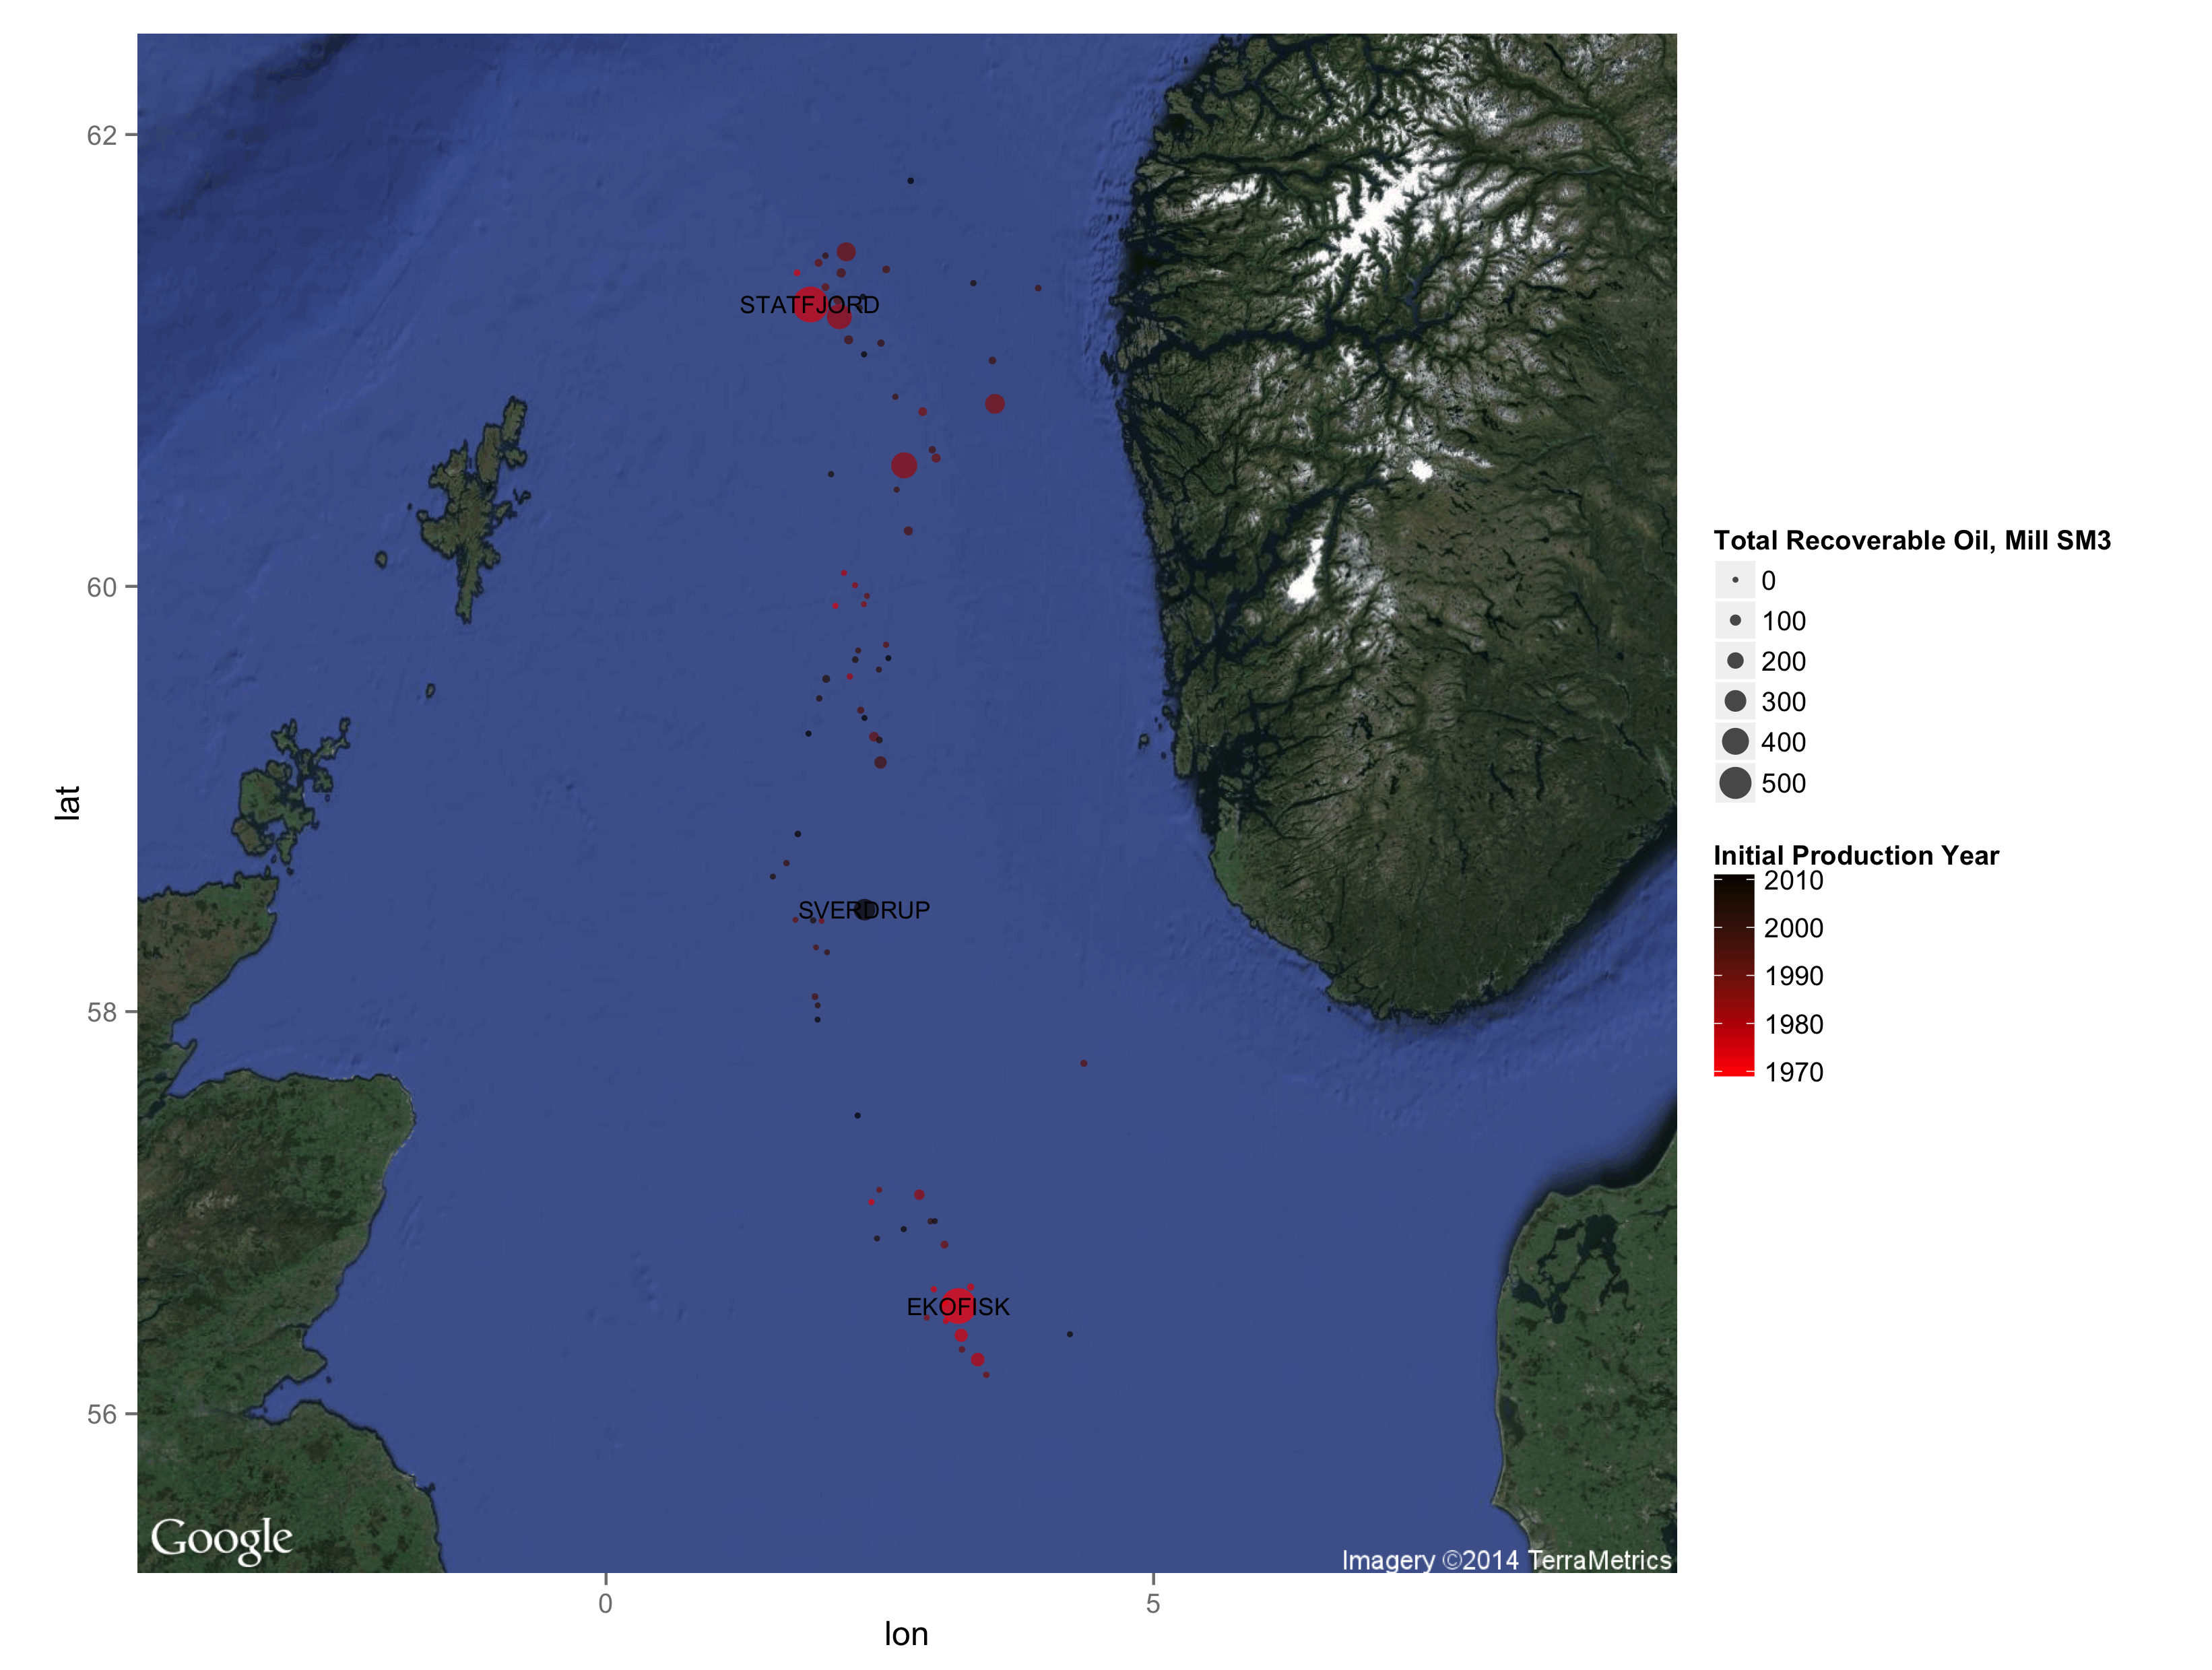
\includegraphics[width=.8\textwidth]{north_sea_reserves.png}
\end{figure}

Exploration in the Norwegian sea was opened up for exploration in 1980 and the first commercial field started production in 1981.  While several mid-sized fields have been discovered, the Norwegian Sea has generally disapointed in terms of commercial oil finds and most finds have been relatively small (figure 3).  
\begin{figure}
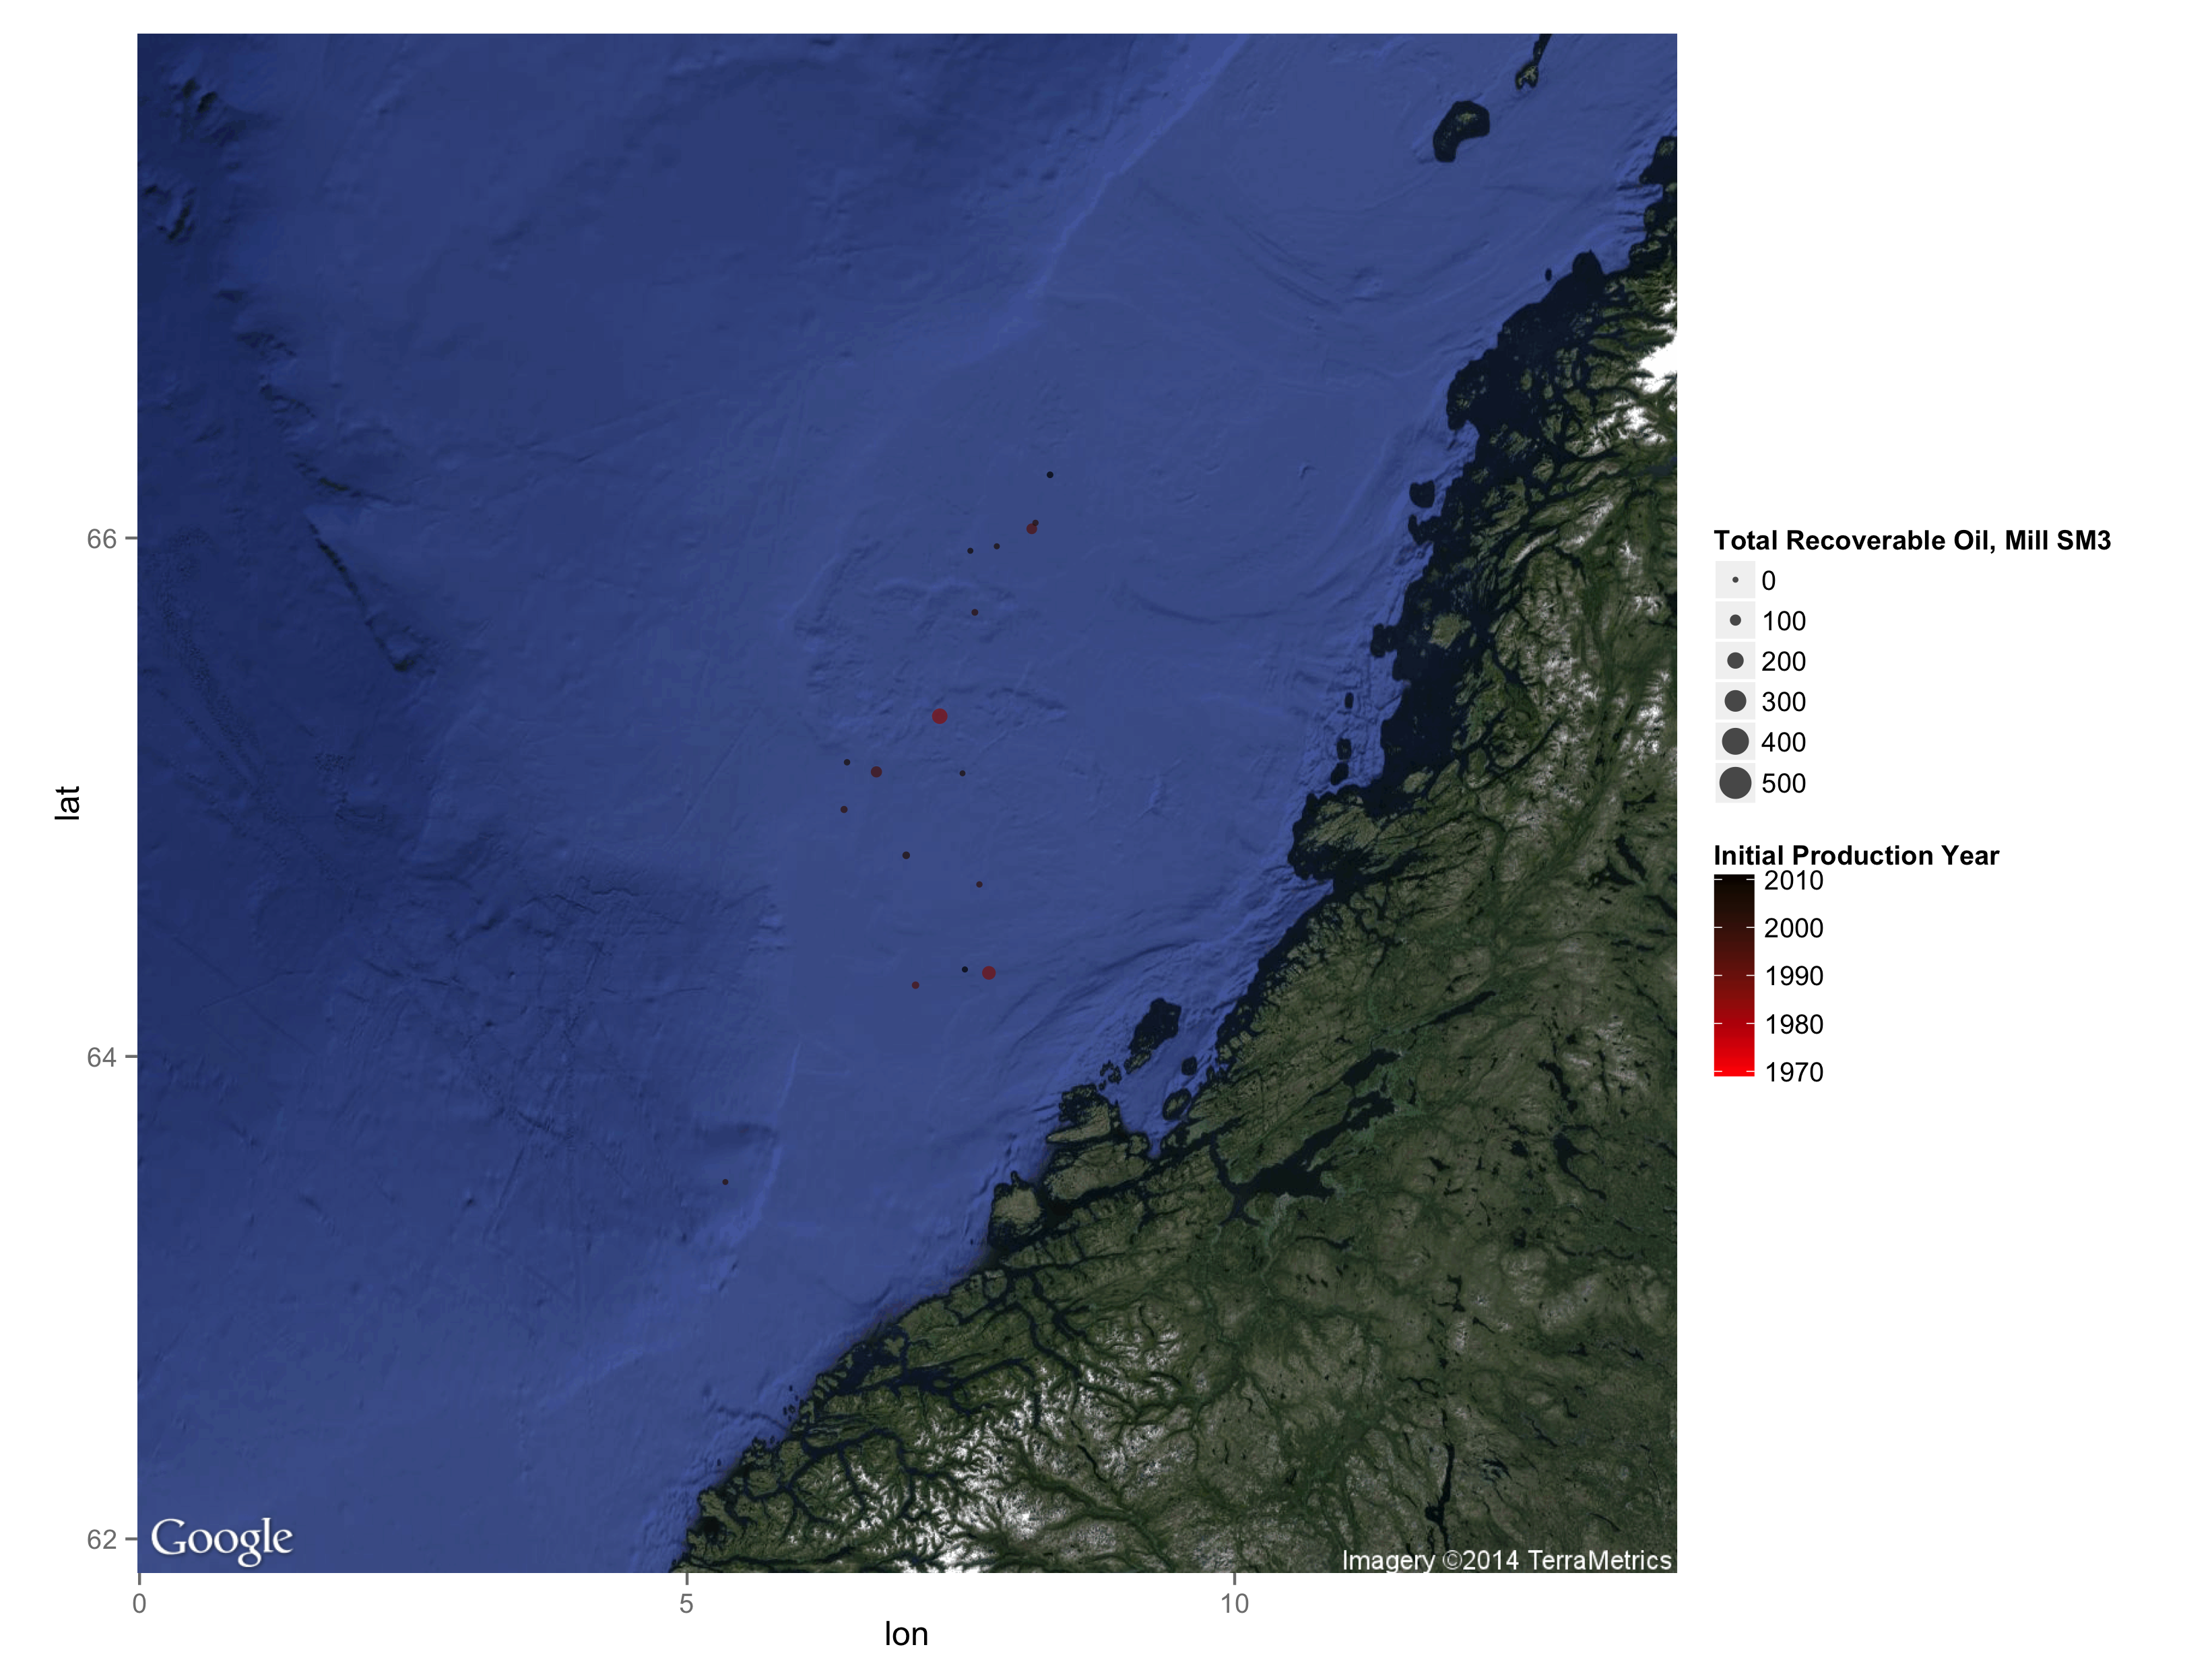
\includegraphics[width=.8\textwidth]{norwegian_sea_reserves.png}
\end{figure}
Norwegian waters in the Barents sea have also been open to exploration since the 1980s, however up until recently only a few, small finds were made and none came into commercial production.  However more recently several large oil and gas finds have been made in the Barents Sea - notably the oil find Goliat and the large gas find Snøhvit, which are both currently under development but not yet producing.  The agreement between Norway and Russia in June 2011 settling a long-running dispute over the maritime delimitation has also given a boost to new exploration in the region.  

\section{Norwegian oil field production data}
Production data of Norwegian oil fields is obtained from the website of the Norwegian Petroleum Directorate \footnote{http://factpages.npd.no/}  Production data is available at a monthly frequency for all fields, though I choose to aggregate up to yearly values both to smooth over seasonality as well as random changes in output.  

In addition to data on field-level production, I also make use of data on estimated total recoverable reserves.  The use of this variable is complicated as it is an estimate subject to a large amount of uncertainty, especially in relatively young fields.  

I use yearly data from the US Energy Information Agency on the real price of Brent-traded oil in 2010 dollars.  The Brent benchmark oil price is likely the best oil price measure for Norwegian production as it is based on light sweet crude oil sourced from the North Sea.   

\section{A generalized additive model of oil field production}
A parametric linear model has the sizeable advantages of simplicity and interpretability and therefore usually a good starting point for an analysis.  However, when attempting to model the effect of price on oil field production, a standard linear model is unable to sufficiently control for the production profile and therefore biasing the estimate of the effect of price.  As an example, consider a generalized linear model written as in equation 1. 

	\begin{equation}
	\begin{split}
	 Log(Production_{i,t}) & = \alpha_0 + \alpha_1 time\_to\_peak_{i,t} + \alpha_2 time\_to\_peak_{i,t}^2 \\
	& \quad + \alpha_3 time\_to\_peak_{i,t}^3  + \alpha_4 peak\_to\_end_{i,t} + \alpha_5 peak\_to\_end_{i,t}^2 \\
	& \quad + \alpha_6 peak\_to\_end_{i,t}^3 + \gamma total\_recoverable\_oil_i \\
	& \quad + \beta_1 oil\_price + \beta_2 oil\_price\_l1 + ...+ \epsilon
	\end{split}
	\end{equation}

Here the left hand side variable is yearly production in year $t$ for field $i$.  To try to account for the time profile of production, I split up model time into a time-to-peak and peak-to-end variable as shown in figure x and then represent each as a cubic function.  The total size of the field will of course also play a role in the production and this is added linearly in the model.  Finally, a term for the oil price as well as 5 lagged terms are added in order to capture the effects of price.  

\begin{figure}
\includegraphics[width=.8\textwidth]{statfjord_dem.png}
\end{figure}

Figure x shows the estimates of the coefficients on the oil price and its lags \footnote{The dots on the figure represent 1000 simulations of the estimated coefficient based on the estimated standard error and point estimate from the model}.  The lags are not estimated to have an affect significantly different from zero. However a literal interpretation of the coefficients would indicate that a 10-dollar increase in the oil price would lead to a lowering of field production of around 2\%.

\begin{figure}
\includegraphics[width=.8\textwidth]{glm_dirty_box.png}
\end{figure}

The estimates are of course heavily biased downwards due to the spurious correlation between the field production profiles and the autocorrelated time series of Brent oil prices.  The parametric representation is not flexible enough to control for the production profile of the fields.  Instead, a more flexible estimation of the production profile is needed. 

Instead of attempting to estimate the shape of the production profiles of the fields by estimating parameters on linear terms I estimate a non-parametric function for the production profile.  As an illustration, consider the production profile of a single field.  The simplest possible model would then have the form of equation x. 

\begin{equation}
Production_{t}=f(time) + \epsilon
\end{equation}

Again considering the production profile for the Statfjord field, a smoothed function might look like the black line in figure x.   

\begin{figure}
	\includegraphics[width=1\textwidth]{statfjord_gam.png}
\end{figure}

In principle any number of well-behaved smoothers could be used to estimate the function, for example a Loess or a kernel smoother.  In practice regression splines are most commonly used.  With a regression spline the data points for the function to be estimated is broken into bins.  For each bin of data a local linear regression is estimated.  For functions of one variable, a cubic parameterization is often used.  These regressions are then essentially tied together at what are called “knots” and the smoothness of the overall function is controlled by a penalty function that consists of the second derivative of estimated function.

The advantage to using splines over other smoothing methods is that it can be represented in a linear form.  Thus estimation of the model can be done by standard and efficient linear algorithms.  Variants of an iterative back-fitting least square procedure is the most common fitting procedure.  For further details I refer to the discussion in \citet{tsibriani90} and \citet{wood04}.  The latter is a particularly useful reference for implementing generalized additive models in R.  As a general note, this paper is not meant as a methodological piece.  The methods used here, while still not common in economics, are mature, developed and commonly used in Statistics as well as by other empirical researchers.

Of course, I do not want to estimate smoothed curves individually for each field.  While this would provide a good overall fit to the full data set, it would not be particularily information.  Instead I want to estimate a general shape of the production profile for all fields and then use the remaining variation in the data to see what effect price has.  My model can be written as in equations x.

\begin{equation}
\begin{split}
	Log(Production_{i,t})&=f(time\_to\_peak_{i,t}, total\_recoverable\_oil_i) \\
	& \quad + f(peak\_to\_end_{i,t}, total\_recoverable\_oil_i) \\
	& \quad + \beta_1 oil\_price + \beta_2 oil\_price\_l1 + ... +  \epsilon
\end{split}
\end{equation}

In this model I am estimating the parameters and functions from all fields $i$. As in the parametric model presented earlier, the left-hand-side variable is yearly oil production for field $i$. Also like the parametric model I split the production-time component element in two -up to and after the peak in production.  While a shape for the entire production profile could be estimated with one smoothed function, splitting it up into two allowed for more flexibility and better overall fit of the model as estimated by deviance score and the related estimated degrees of freedom of the model \citet[p.xx]{wood04}.  

 I also allow the smoothed functions to vary with the total size of the field as measured by the estimated total recoverable oil since the shape of the production profile tends to vary substantially by field size.  Inspection of a selection of fields, such as shown in figure x, shows that smaller fields tend to reach their peak quickly while larger fields, which need to be built up in order to reach their full production, take more time.   Such a two-dimensional function can not be estimated by a traditional cubic regression spline.  Instead what is referred to as a thin-plate spline is used to estimate the smoothed functions….


\begin{figure}
	\includegraphics[width=1\textwidth]{field_inspection.png}
\end{figure}

Even with a smoothed function that is allowed to vary by field-size, a substantially better fit could be attained by splitting the estimation into small and large fields, this time measured by max production year.  The improvement in fit can be seen by inspecting the fitted values of the models as in figure x. The split estimation provides a particularly better fit for smaller and mid-sized fields.

\begin{figure}
	\includegraphics[width=1\textwidth]{bench_vs_split.png}
\end{figure}

The variables of interest is of the course the oil price, which I include as a linear parametric term in the model.  I also include six lags of the oil price variable in the model, again as linear parametric terms.  The idea of including both a concurrent oil price term as well as lags is that a change in price could conceivably have two effects on oil production in a field.  First, the field operator could be operating on the basis of some short-term extraction rule - choosing to pump out less at times of lower prices so that they could pump out more at periods of high prices.  

Alternatively, a change of oil prices can be seen as a lifting of a production constraint.  A higher oil price means that is worthwhile to invest more in production, increasing the current rate of production and potentially leading to an overall higher extraction rate.  

The estimates of the parametric oil price terms are shown in figure x.

\begin{figure}
	\includegraphics[width=1\textwidth]{gam_price_under_dirty_box.png}
\end{figure}

%\begin{figure}
%	\includegraphics[width=1\textwidth]{gam_price_over_dirty_box.png}
%\end{figure}



	a. Getting a causal interpretation on the coefficient of the oil price variable
		-oil is globally 
	b. comparison to the ideal experiment.  
	To clearify the discussion of causality as well as the limitations of this study I find it useful to describe a hypothetical ideal experiment (as suggested by Gelman and Hill 2007)






\bibliographystyle{abbrv}
\bibliography{main}

\end{document}
This is never printed